%%%%%%%%%%%%%%%%%%%%%%%%%%%%%%%%%%%%%%%%%
% Beamer Presentation
% LaTeX Template
% Version 1.0 (10/11/12)
%
% This template has been downloaded from:
% http://www.LaTeXTemplates.com
%
% License:
% CC BY-NC-SA 3.0 (http://creativecommons.org/licenses/by-nc-sa/3.0/)
%
%%%%%%%%%%%%%%%%%%%%%%%%%%%%%%%%%%%%%%%%%

%----------------------------------------------------------------------------------------
%	PACKAGES AND THEMES
%----------------------------------------------------------------------------------------

\documentclass{beamer}

\mode<presentation> {

% The Beamer class comes with a number of default slide themes
% which change the colors and layouts of slides. Below this is a list
% of all the themes, uncomment each in turn to see what they look like.

%\usetheme{default}
%\usetheme{AnnArbor}
%\usetheme{Antibes}
%\usetheme{Bergen}
%\usetheme{Berkeley}
%\usetheme{Berlin}
%\usetheme{Boadilla}
%\usetheme{CambridgeUS}
%\usetheme{Copenhagen}
%\usetheme{Darmstadt}
%\usetheme{Dresden}
%\usetheme{Frankfurt}
%\usetheme{Goettingen}
%\usetheme{Hannover}
%\usetheme{Ilmenau}
%\usetheme{JuanLesPins}
%\usetheme{Luebeck}
\usetheme{Madrid}
%\usetheme{Malmoe}
%\usetheme{Marburg}
%\usetheme{Montpellier}
%\usetheme{PaloAlto}
%\usetheme{Pittsburgh}
%\usetheme{Rochester}
%\usetheme{Singapore}
%\usetheme{Szeged}
%\usetheme{Warsaw}

% As well as themes, the Beamer class has a number of color themes
% for any slide theme. Uncomment each of these in turn to see how it
% changes the colors of your current slide theme.

%\usecolortheme{albatross}
%\usecolortheme{beaver}
%\usecolortheme{beetle}
%\usecolortheme{crane}
%\usecolortheme{dolphin}
%\usecolortheme{dove}
%\usecolortheme{fly}
%\usecolortheme{lily}
%\usecolortheme{orchid}
%\usecolortheme{rose}
%\usecolortheme{seagull}
%\usecolortheme{seahorse}
%\usecolortheme{whale}
%\usecolortheme{wolverine}

%\setbeamertemplate{footline} % To remove the footer line in all slides uncomment this line
%\setbeamertemplate{footline}[page number] % To replace the footer line in all slides with a simple slide count uncomment this line

%\setbeamertemplate{navigation symbols}{} % To remove the navigation symbols from the bottom of all slides uncomment this line
}

\usepackage{graphicx} % Allows including images
\usepackage{booktabs} % Allows the use of \toprule, \midrule and \bottomrule in tables

%----------------------------------------------------------------------------------------
%	TITLE PAGE
%----------------------------------------------------------------------------------------

\title[Analisis Numerik]{Analisis Numerik} % The short title appears at the bottom of every slide, the full title is only on the title page

\author{Ahmad Rio Adriansyah} % Your name
\institute[STT-NF] % Your institution as it will appear on the bottom of every slide, may be shorthand to save space
{
STT Terpadu - Nurul Fikri \\ % Your institution for the title page
\medskip
\textit{ahmad.rio.adriansyah@gmail.com
\\arasy@nurulfikri.ac.id} % Your email address
}
\date{\today} % Date, can be changed to a custom date

\usepackage{graphicx}
\begin{document}

\begin{frame}
\titlepage % Print the title page as the first slide
\end{frame}

%----------------------------------------------------------------------------------------
%	PRESENTATION SLIDES
%----------------------------------------------------------------------------------------

%------------------------------------------------

\begin{frame}
\frametitle{Analitik vs Numerik}
Contoh : Bagaimana menghitung nilai $x$ yang memenuhi persamaan $x^2+4x-5=0$ ?
\\\ \\
Analitik :
\\1. Pemfaktoran
\\2. Kuadrat Sempurna
\\3. Formula Al Khawarizmi
\end{frame}

%------------------------------------------------

\begin{frame}
\frametitle{Analitik vs Numerik}
Keuntungan solusi analitik :
\begin{itemize}
\item Nilai perhitungannya sejati (exact)
\item Solusi dapat berbentuk angka atau fungsi matematik
\end{itemize}
\ \\\ \\
Kekurangan solusi analitik :
\begin{itemize}
\item Memakan banyak waktu, tenaga, dan pikiran
\item Solusi tidak selalu dapat ditemukan 
\end{itemize}

\end{frame}

%------------------------------------------------

\begin{frame}
\frametitle{Analitik vs Numerik}
\begin{equation}
\int_{-2,75}^{\pi} \sqrt[3]{\dfrac{20,3x^{16}}{ln(cos(x))}+e^{2x}} dx
\nonumber
\end{equation}
\ \\\ \\\ \\\ \\\qquad \qquad \quad Bagaimana mencari solusi untuk permasalahan ini\\\qquad \qquad \quad secara analitik?
\end{frame}

%------------------------------------------------

\begin{frame}
\frametitle{Analitik vs Numerik}
Metode Numerik = Teknik yang digunakan untuk memformulasikan persoalan matematik sehingga dapat dipecahkan  dengan operasi aritmatika biasa (tambah, kurang, kali, bagi)
\end{frame}

%------------------------------------------------

\begin{frame}
\frametitle{Analitik vs Numerik}
Keuntungan solusi numerik :
\begin{itemize}
\item Dapat diserahkan pengerjaannya ke komputer
\item Dapat memecahkan persoalan yang tidak dapat dipecahkan dengan metode analitik
\item Perhitungannya sederhana (hanya tambah, kurang, bagi, kali)
\end{itemize}
\ \\\ \\
Kekurangan solusi numerik :
\begin{itemize}
\item Solusi hanya dapat berbentuk angka
\item Solusi yang dihasilkan merupakan hampiran (mengandung error)
\item Perhitungannya lama dan berulang-ulang
\end{itemize}

\end{frame}

%------------------------------------------------

\begin{frame}
\frametitle{Aplikasi Numerik}
\begin{itemize}
\item Menyelesaikan problem matematika
\\\quad $->$ Sistem Persamaan Linier 
\\\quad $->$ Regresi Linier
\\\quad $->$ Interpolasi
\\\quad $->$ Integral dan Turunan
\item Simulasi kejadian alam (kebakaran, tsunami)
\item Desain produk 
\item Teknik dan rekayasa
\end{itemize}

\end{frame}

%----------------------------------------------------------------------------------------

\begin{frame}
\frametitle{Aplikasi Numerik}
\begin{figure}[htp]
\centering
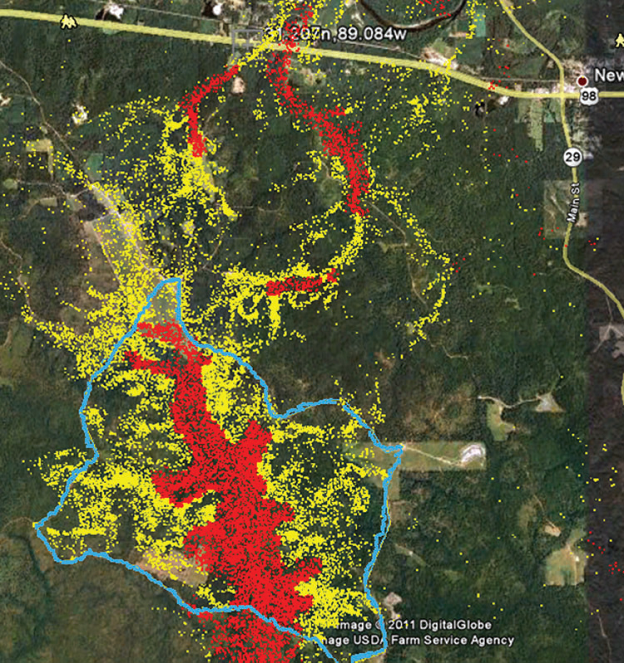
\includegraphics[scale=0.40]{ditempel201.png}
\end{figure}
\end{frame}

%----------------------------------------------------------------------------------------

\begin{frame}
\frametitle{Aplikasi Numerik}
\begin{figure}[htp]
\centering
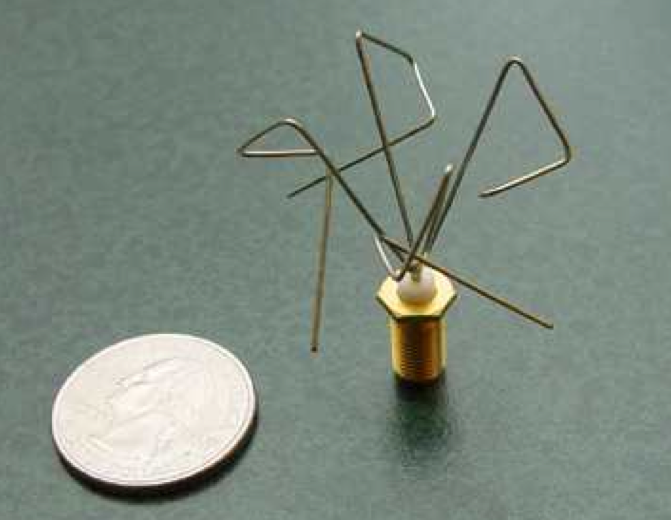
\includegraphics[scale=0.30]{2v2aww6.png}
\end{figure}
\end{frame}
%----------------------------------------------------------------------------------------

\begin{frame}
\frametitle{Aplikasi Numerik}
\begin{figure}[htp]
\centering
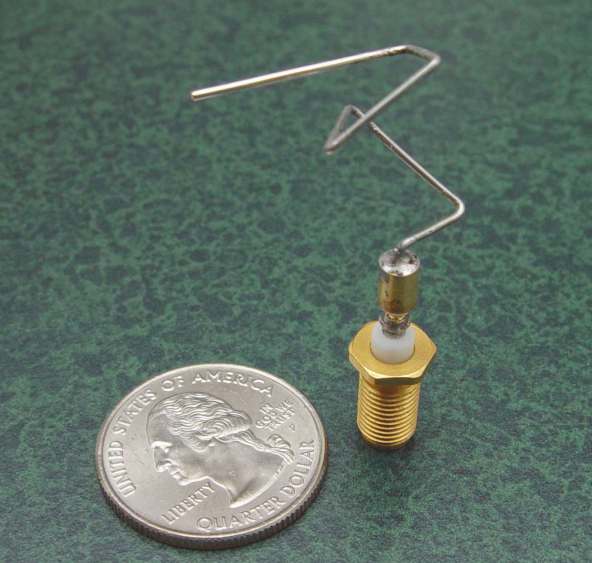
\includegraphics[scale=0.30]{9sh549.png}
\end{figure}
\end{frame}
%----------------------------------------------------------------------------------------
\begin{frame}
\frametitle{Permasalahan dalam Analisis Numerik}
\begin{itemize}
\item Masalah keberadaan dari solusi (\textit{Existence})
\item Seberapa bagus hampiran kita? (\textit{Error Analysis})
\item Seberapa efisien metode kita? (\textit{Algorithm Design, Convergence Rate})
\item Apakah metode kita selalu berhasil? (\textit{Convergence})
\end{itemize}
\end{frame}

%----------------------------------------------------------------------------------------
\begin{frame}
\frametitle{Penyelesaian Masalah dengan Numerik}
\begin{itemize}
\item Pemodelan
\\Mengubah permasalahan dunia nyata ke dalam persamaan matematis
\item Penyederhanaan Model
\item Formulasi Numerik
\\Menentukan metode numerik yang akan digunakan, analisis galat awal, dan menyusun algoritma
\item Pemprograman
\item Operasional
\\Menguji program dengan data
\item Evaluasi
\\Menerjemahkan hasil yang didapat ke dalam persoalan nyata kembali
\end{itemize}
\end{frame}


\begin{frame}
\frametitle{Peranan Komputer}
\begin{quote}
Computers are incredibly fast, accurate, and stupid. Human beings are incredibly slow, inaccurate, and brilliant. Together they are powerful beyond imagination. 
\\\qquad \qquad \qquad \qquad \qquad \qquad \qquad \qquad \qquad Albert Einstein
\end{quote}
\end{frame}

%----------------------------------------------------------------------------------------

\begin{frame}
\frametitle{Peranan Komputer}
\begin{figure}[htp]
\centering

\includegraphics[scale=0.50]{theory-is-when-you-know-everything-but-nothing-works.jpg}
\end{figure}
\end{frame}

%----------------------------------------------------------------------------------------

\begin{frame}
\frametitle{Peranan Komputer}
Komputer digunakan untuk :
\begin{itemize}
\item Memprogram
\item Mempercepat perhitungan 
\item Mencoba berbagai kemungkinan solusi akibat perubahan parameter
\item Meningkatkan ketelitian (mengurangi error/galat)
\end{itemize}
\end{frame}

%----------------------------------------------------------------------------------------
\begin{frame}
\frametitle{Galat}
Berdasarkan perhitungannya, galat dibagi 2 :
\begin{itemize}
\item Galat pemotongan (\textit{truncation error})
\item Galat pembulatan (\textit{round-off error})
\end{itemize}
\ \\\ \\
Berdasarkan sumbernya, galat dibagi lagi, antara lain :
\begin{itemize}
\item Galat pemodelan
\\galat akibat salah memodelkan atau penggunaan asumsi
\item Galat eksperimental 
\\galat akibat kesalahan pengukuran, ketidaktelitian alat, dsb.
\item Galat pemprograman 
\\kesalahan pada program yang tidak diharapkan (\textit{bug})
\end{itemize}
\end{frame}

%----------------------------------------------------------------------------------------
\begin{frame}
\frametitle{Deret Taylor dan Deret Maclaurin}
Deret Taylor\\\ \\
$f(x) = f(x_0)+ \dfrac{(x-x_0)}{1!}f'(x_0) + \dfrac{(x-x_0)^2}{2!}f''(x_0) + \dfrac{(x-x_0)^3}{3!}f'''(x_0) + \dots $
\\\ \\\ \\\ \\Deret Maclaurin = Deret Taylor baku, dengan $x_0=0$\\\ \\
$f(x) = f(0)+ \dfrac{x}{1!}f'(0) + \dfrac{x^2}{2!}f''(0) + \dfrac{x^3}{3!}f'''(0) + \dots $

\end{frame}

%----------------------------------------------------------------------------------------
\begin{frame}
\frametitle{Galat Pemotongan}
Contoh : Nilai $cos(x)=1-\dfrac{x^2}{2!}+\dfrac{x^4}{4!}-\dfrac{x^6}{6!}+\dfrac{x^8}{8!}-\dfrac{x^{10}}{10!}+\dfrac{x^{12}}{12!}-\dots$
\\\ \\$cos(x)\approx \underbrace{1-\dfrac{x^2}{2!}+\dfrac{x^4}{4!}-\dfrac{x^6}{6!}}_{\text{Nilai hampiran}}+ \Biggl\{\underbrace{\dfrac{x^8}{8!}-\dfrac{x^{10}}{10!}+\dfrac{x^{12}}{12!}-\dots }_{\text{Galat pemotongan}}\Biggr\}$
\\\ \\$cos(x)\approx {1-\dfrac{x^2}{2!}+\dfrac{x^4}{4!}-\dfrac{x^6}{6!}} + \epsilon$ 
\end{frame}

%----------------------------------------------------------------------------------------
\begin{frame}
\frametitle{Galat Pembulatan}
Contoh : Nilai $\dfrac{10}{3} = 3,3333333...$
\\\ \\Komputer hanya mampu merepresentasikan sejumlah digit. Bilangan real yang panjangnya melebihi jumlah digit (bit) yang dapat direpresentasikan oleh komputer dibulatkan ke bilangan terdekat.
\\\ \\$\dfrac{10}{3} \approx \underbrace{3,3333}_{\text{Nilai hampiran}} + \underbrace{0,0000333...}_{\text{Galat pembulatan}}$
\end{frame}

%----------------------------------------------------------------------------------------

\end{document} 